\documentclass[a4paper,10pt]{article}
\usepackage[spanish]{babel}
\usepackage[utf8]{inputenc}
\usepackage{hyperref}
\usepackage{multicol}
\usepackage{geometry}
\usepackage{graphicx}
\newcommand*{\airbnb}{\textit{Airbnb}}
\newcommand*{\webscrapping}{\textit{web scrapping}}

\geometry{
    a4paper,
    total={170mm,257mm},
    left=20mm,
    top=20mm,
    }

\title{Alquiler Turístico en España y Sevilla}
\author{Mario Pantoja Castro}
\date{Abril 2023}

\begin{document}

    \maketitle

    \begin{abstract}
       hola blabllbalbllalblalalblablbalbla
    \end{abstract}

    \vspace{3mm}

    \begin{multicols}{2}
    
        \section{Introducción}

            \paragraph*{}
            El sector turístico constituye una de las más importantes fuentes de ingresos en la economía española. Así es tambíen en las economías de Andalucía y
            Sevilla. De tal manera ha sido desde el desarrollo turístico que experimentó el pais durante el tardofranquismo y las décadas posteriores. Sin embargo, 
            recientemente y gracias a la llegada de la revolución digital se han desarrollado nuevas y diversas formas de turismo. Otras se han visto favorecidas
            por el poder de difusión y alcanze que las nuevas tecnologias nos ofrecen. Es el caso del alquiler vacacional, es decir, el alquiler de inmuebles a
            corto o medio plazo con fines turísticos. La importancia que este sector tiene y que año tras año se va incrementando en el turismo nacional hace de 
            su estudio una labor interesante.
            
            \paragraph*{}
            Asimismo, a causa de la pandemia por coronavirus, el alquiler turístico se vio mermado en su totalidad, 
            provocando adversos efectos económicos. Tras esta situación su crecimiento fue exponencial, volviendo a recuperar e incluso incrementar la importancia
            que había tenido para el turismo y la economía en general.

            \paragraph*{}
            Por otro lado, este rápido crecimiento del sector del alquiler turístico, tanto en España o como en el resto del mundo, se debe en gran parte al 
            desarrollo y crecimiento de empresas digitales tales como \textit{Airbnb, Booking} o \textit{Vrbo} que facilitan las relaciones entre
            arrendador y arredatario al ofrecer plataformas donde anunciar y alquilar inmuebles de manera segura.

            \paragraph*{}
            No obstante, a pesar del gran impacto que este negocio supone en el sector turístico general, y a su vez en la economía, el hecho de que se
            produzca en Internet y a través de empresas privadas dificulta la tarea de recopilación de datos estadísticos sobre el mismo. Por esta razón,
            existe una gran desinformación sobre el alquiler turístico y lo que supone para la economía frente a otros sectores del turismo.
            \vfill\null

            \columnbreak
            \paragraph*{}
            En este contexto, el presente trabajo se propone arrojar luz sobre los datos más importantes de alquiler turístico a nivel nacional, autónomico y 
            provincial; haciendo especial hincapié en la ciudad de Sevilla, donde se pretende hacer un estudio más pormenorizado. 

        \section{Descripción de los objetivos}

            \paragraph*{}
            Motivado por la dificultad de obtener información clara y fiable sobre el alquiler turístico de manera desagregada,
            el principal objetivo del texto es presentar datos estadísticos que permitan realizar comparaciones entre los distintos
            territorios del estado español sobre el tema en cuestión.
            
            \paragraph*{}
            En concreto, se pretende analizar y comparar los precios del alquiler turístico a nivel nacional, según comunidades 
            autónomas; a nivel andaluz, según provincias; y en torno a la ciudad de Sevilla, según distritos. Se quiere también estudiar los diferentes tipos de 
            inmueble que se ofrecen en alquiler turístico y la distribución de los anuncios de los arredadores, es decir, la densidad de éstos, por las áreas 
            descritas anteriormente. Por último, se busca obtener resultados sobre la evolución del sector en cuestión tras la pandemia COVID, así como 
            comparar de que manera se ha visto afectado por esta situación frente a indicadores como el Índice de Precios al Consumo (IPC).
       
        \clearpage
        \section{Metodología y desarrollo de la investigación}

            \paragraph*{}
            Para el proceso de investigación del presente trabajo se han utilizado herramientas puramente informáticas. Con el fin de que se entienda cómo y 
            porqué se ha llevado a cabo el estudio de esta manera, se expondrán las distintas fases de la investigación detallando en cada una de ellas los recursos 
            informáticos utilizados y la justificación correspondiente. Se adelanta que los datos a partir de los cuales se ha realizado el estudio se dividen
            en tres grandes conjuntos:

            \begin{itemize}
                    
                \item[-] Datos relativos al alquiler turístico en Sevilla (2017-2018)
                \item[-] Datos relativos al alquiler turístico en España (2017-2018)
                \item[-] Datos relativos al alquiler turístico en Sevilla (2022)
            
            \end{itemize} 

            \paragraph*{\textbf{Fase 1: Recopilación de datos.}}
            Existen muy pocas fuentes fiables que aporten datos sobre el alquiler turístico de manera desagregada, esto es, 
            por sectores territoriales como provincias o distritos.
            Como se comentó en la introducción, la obtención de datos sobre el tema, y más aún aquellos de carácter desagregado, es limitada, complicada
            y costosa. Esto se debe mayoritariamente a que el negocio del alquiler turístico se lleva a cabo casi en su totalidad vía páginas webs de empresas
            privadas. Éstas no ponen a disposición pública los valiosos datos que poseen sino que, bajo circunstancias muy específicas, ceden parte de ellos, imposibilitanto al que lo recibe la difusión de los mismos. En la mayoría de los casos, estos datos se compran directamente a las empresas privadas para 
            la realización de un estudio en particular pero, por supuesto, solo pudiendo publicar conclusiones sacadas a raíz de los datos en disposición y no éstos 
            de manera explícita. \\

            \noindent
            Sin embargo, existe una herramienta informática a través de la cual se puede obtener información, aunque con limitaciones, de manera legal.
            Se trata del \textit{web scraping}. Esta herramienta permite al que la usa obtener grandes cantidades de datos expuestos en una página web.
            En nuestro caso, la página web en cuestión es \textit{Airbnb}. \footnote{Aunque se podían haber usado datos procedentes de diferentes webs, 
            se ha preferido usar solo los datos de una única web puesto que muchos arredadores publicitan sus anuncios en diferentes plataformas, lo que hubiese 
            ocasionado datos redundates. La elección de \airbnb \ se debe al gran volumen de datos que ofrece y a la importancia que tiene en el sector.} \\
           
            \noindent
            Intuitivamente, el \textit{web scraping} permite rastrear los datos que aparecen 
            en una web pero que por su gran magnitud resultaría imposible realizar manualmente. 
            \vfill\null
            
            \columnbreak
            \noindent
            Por ejemplo, en nuestra situación, las técnicas descritas 
            permiten obtener datos relativos al precio, lugar, fecha y demás características relativas a los anuncios publicitarios expuestos en \airbnb. \\
        
            \noindent
            De esta manera se han obtenido todos los datos que se han usado en el proceso de investigación del trabajo. Ahora bien, aunque con la misma técnica
            del \webscrapping, son tres las fuentes de datos de las que se han hecho uso. Por un lado, los datos de alquiler turístico ofrecidos por 
            \airbnb \  relativos a Sevilla y a España en general de los años 2017 - 2018 se han obtenido de \cite{datahippo}. Por otro, los datos 
            de Sevilla del año 2022 son de \cite{insideairbnb} que, a su vez, han sido complementados con otros datos resultantes de un \textit{scraping} personal.
            \footnote{Los datos que ofrecía \cite{insideairbnb} eran incompletos y no los suficientemente útiles para el estudio que el autor quería hacer. Por ello,
            se llevó a cabo un \textit{scraping} para aumentar la información de los anuncios de \airbnb \ que la web citada ponía a disposición. No se 
            entrará en detalles sobre las técnicas informáticas utilizadas pero se pondrá a disposicón los ficheros de datos (CSV) que se obtuvieron.} 

            \paragraph*{\textbf{Fase 2: Limpieza de datos.}}
            Una vez obtenidos los \textit{datasets}, el proceso de limpieza y depuración de éstos, es decir, la clasificación de los datos, eliminación de 
            anomalias, obtención de nueva información a partir de la disponible y, en definitiva, todo lo necesario para posteriormente obtener estadísticas 
            y graficas fiables y valiosas; se ha realizado a través del lenguaje de programación \emph{Python} y, más concretamente, a través de una librería 
            auxiliar de éste llamada \emph{Pandas}. \\
            Sin entrar en detalles técnicos, los criterios bajo los cuales se ha realizado la limpieza de datos son:

            \begin{enumerate}
                \item Anuncios proveídos por \airbnb \ y no por otra web de alquiler turístico
                \item Anuncios con \textit{reviews} en el último año y no aquellos que no tienen ninguna
                \item Anuncios con ninguna característica nula. Se deshechan, por ejemplo, anuncios que no tengan precio o capacidad.  
            \end{enumerate}

            \noindent
            Finalmente, los datos que quedaban se han truncado bajo criterios estadísticos. Esto es, se han eliminado aquellos anuncios que, en relación al
            precio y al tipo de inmueble que ofrecían, no estaban dentro de los margenes cuantílicos (\textit{outliers}). Es decir, aquellos que no estaban entre
            el cuantil 003 y el cuantil 097 según el precio por noche. \\

            \noindent
            Así, la muestra de datos de la investigación la constituyen aquellos anuncios que cumplen los criterios descritos anteriormente y que 
            pertenecen a los \textit{datasets} considerados en la Fase 1.

            \clearpage
            \paragraph*{\textbf{Fase 3: Obtención de estadísticas y gráficas.}}
            Finalmente, los resultados estadísticos así como todas las gráficas que figuran en 
            el texto, a menos que se exprese lo contrario, se han obtenido nuevamente con \emph{Python}, concretamente con las librerías anexas \emph{Pandas, 
            Matplotlib} y \emph{Seaborn}. Una vez más, no se entrará en detalles técnicos, pero se dirá que se ha tratado de exponer los datos de la manera más 
            clara y leal posible a la información obtenida en el proceso de investigación. \\

            \noindent
            Se ha de mencionar que como se asegura la obtención de las graficas, los datos y la limpieza de los mismos con técnicas infórmaticas realizadas por el 
            propio autor, se ha puesto a disposición del lector un repositorio de código (\hyperlink{github}{[GitHub]}) en el \hyperlink{anexo}{Anexo} 
            del texto donde se puede constatar y consultar todo el proceso de investigación que se ha llevado a cabo desde la Fase 2 así como disponer de los conjuntos de datos que se mencionan. Se anima al lector a que consulte dicho repositorio, al menos para comprobar la veracidad de lo expuesto     anteriormente.

    \end{multicols}
        
    \section{Resultados y discusión}

    %       Resultados. Descripción e interpretación del conjunto de información procedente de la parte empírica.
    %       Discusión. Análisis de los resultados tomando como referencia las aportaciones derivadas de la revisión bibliográfica y otros
    %       estudios realizados sobre la temática

        \subsection{Resultados relativos a la distribución de la oferta y a la actividad publicitaria}
            
            \begin{figure}[h]
                \centering
                \includegraphics*[width = 15cm]{graphics/spainccaadensity.png}
            \end{figure}

            \clearpage

            \begin{figure}[h]              
                \centering
                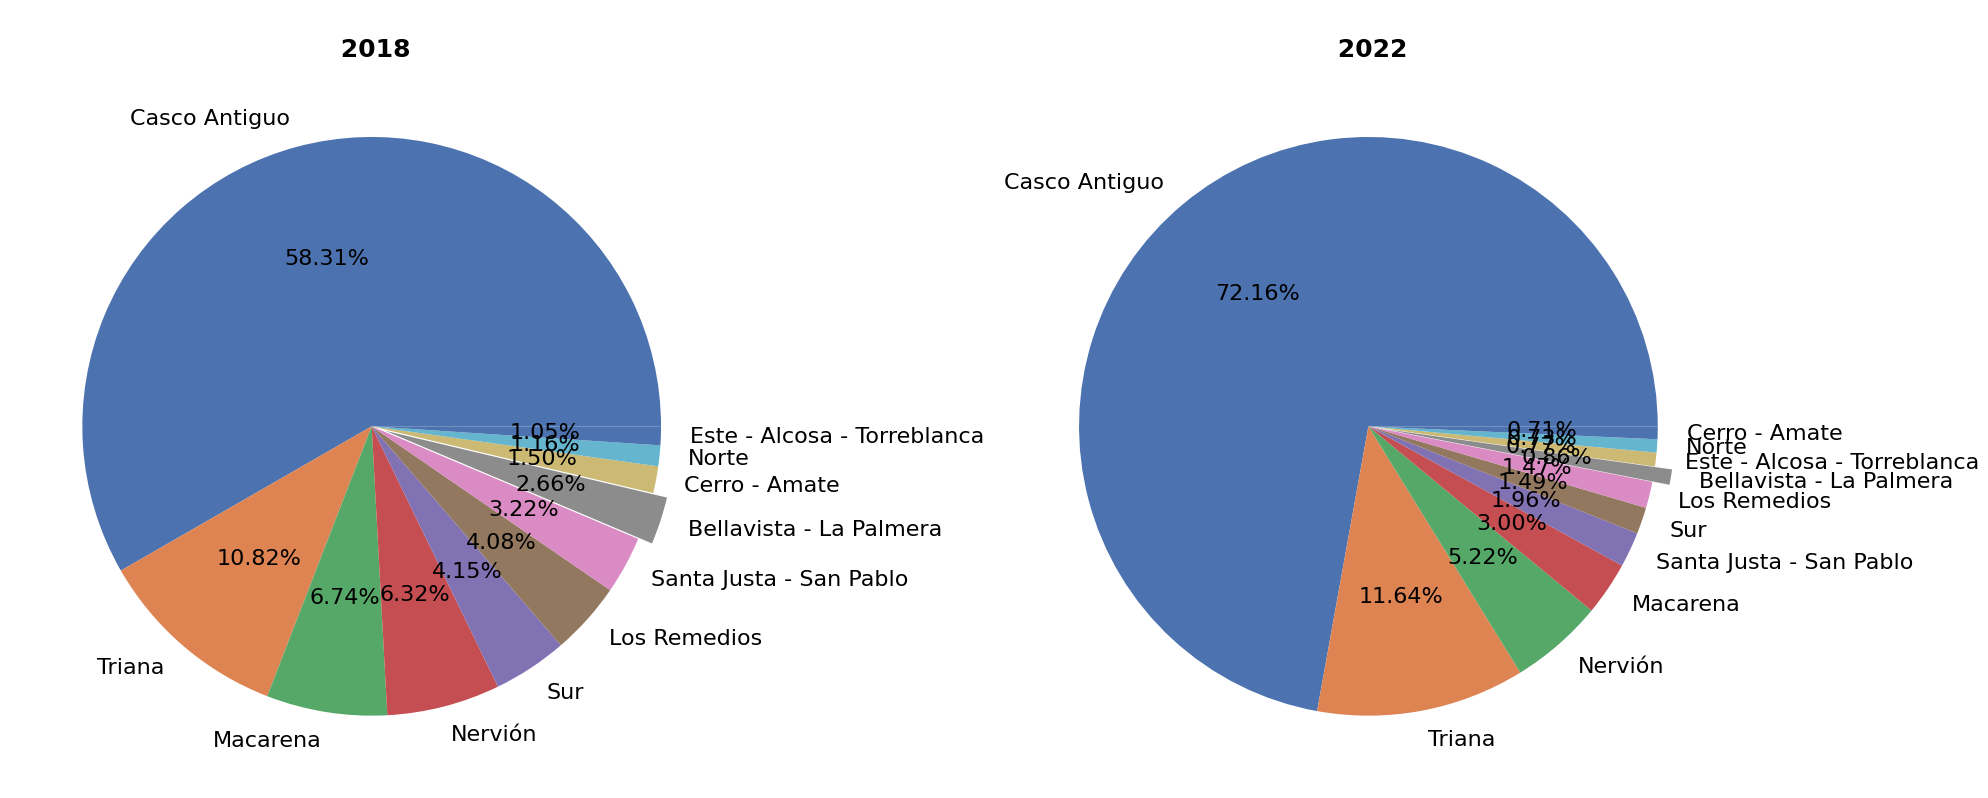
\includegraphics[width = 184mm]{graphics/sevilledensity.png}

            \end{figure}

            






















    % \section{Conclusiones}

    \clearpage
    \begin{thebibliography}{20}

        \bibitem[DataHippo]{datahippo} 
            \ 
            \begin{enumerate}
                \item \href{https://datahippo.org/es/region/599216cb8a4655339b819813/}{Datos España 2017 - 2018}
                \item \href{https://datahippo.org/es/region/599230af8a46554edf884651/}{Datos Sevilla 2017 - 2018}
                \item \href{https://datahippo.org/media/regions/58612732-b2dc-433b-ab78-b8fbe5bbbb16/599216cb8a4655339b819813_airbnb.csv}{Datos España 2017 - 2018 (CSV)}
                \item \href{https://datahippo.org/media/regions/7e3f7365-8ec0-42f1-a277-9b82743b8a39/599230af8a46554edf884651_airbnb.csv}{Datos Sevilla 2017 - 2018 (CSV)}
            \end{enumerate}
        
        \bibitem[InsideAirbnb]{insideairbnb}
            \
            \begin{enumerate}
                \item \href{http://insideairbnb.com/get-the-data/}{Datos Sevilla 2022}
                \item \href{http://data.insideairbnb.com/spain/andaluc%C3%ADa/sevilla/2023-03-31/visualisations/listings.csv}{Datos Sevilla 2022 (CSV)}
            \end{enumerate}

    \end{thebibliography}
    
    \hypertarget{anexo}{}
    \section*{Anexo}

        \hypertarget{github}{[GitHub] \href{https://github.com/m7pantoja/TouristRental}{Repositorio de código sobre el proceso de investigación}}

\end{document}